\chapter{Results}
\label{chapter3}

\section{Evaluation Strategy}

As outlined in the introduction, the focus of this report is on showing how PBS produces more photorealistic images than Blinn-Phong shading. This is fulfilled by highlighting physical phenomena that are modelled more accurately in frames rendered using PBS, than in frames rendered using Blinn-Phong shading. Two such physical phenomena are identified below, and subsequent comparisons performed for each using the application developed.

The first phenomena is the Fresnel effect. Mentioned in section \ref{FresnelReflectance}, the Fresnel effect is the observation that a surface becomes more specular at glancing incident light angles. Faul shows that the Fresnel effect is a key contributor to the appearance of specular materials~\cite{FaulInfluenceOfFresnelEffect}. This suggests that the realism of a shading model is influenced by the degree to which it models the impact of the Fresnel effect. Therefore, it forms a suitable candidate for comparison. In an effort to further build on Faul's investigation, comparing the presence of the Fresnel effect is done by considering the impact it has on the appearance of diffuse materials, rather than specular.

The second physical phenomena is the effect that multiple incoming lights have on the appearance of an object. In the real world, the more lights that are incident to an object, the brighter the object will appear. A comparison is performed between the two shading models to ascertain how accurately they depict how a varying number of point lights influence the appearance of an object.

The evaluation is also supplemented with an analysis of frame times. This assesses whether the implemented shading models are indeed sufficiently performant to be used in real time rendering.

\section{Fresnel Effect Comparison}

\subsection{Testing Method}

Testing a shading model's ability to capture the Fresnel effect could be done using a single point light that is incident to an xz-aligned plane. From a constant viewpoint, the point light could then be moved over the plane so as to vary the incident light angle. From that viewpoint, the amount of specular reflection could be observed. 

However, the test given here is instead performed by keeping the position of the point light constant, and varying the viewing angle (which is also given in respect to the surface normal). The effect of varying the viewing angle is to vary \begin{math}\vect{v}\end{math}, and thus also vary \begin{math}\vect{h}\end{math}; varying \begin{math}\vect{h}\end{math} is equivalent to varying the normals of the microfacets that contribute to the specular reflection; varing the normals has the effect of varying the incident light angle on those microfacets. Although this sequence of implications is certainly complex, carrying out the test in this manner is simpler than the alternative approach given above. Shirley et al present a case study that captures the Fresnel effect by also varying the viewing angle~\cite{PractitionersReflectionModels}. Moreover, as Figure \ref{fig:FresnelRealLife} shows, this testing approach is justified by conducting observations of the real world: the Fresnel effect causes surfaces to appear more specular at glancing viewing angles.

For the tests, two scenes have been created. One for the Blinn-Phong renderer, and another for the physically based renderer. Each scene is arranged in the same manner. A diffuse wooden floor is situated at the origin, and a point light is placed just above it. Four viewing angles are considered, \begin{math}0^{\circ}\end{math}, \begin{math}40^{\circ}\end{math}, \begin{math}65^{\circ}\end{math} and \begin{math}80^{\circ}\end{math}. For each of these angles, the outputted frames of the two renderers are sampled. A shading model that captures the Fresnel effect is expected to render the floor with greater specularity as the viewing angle increases (becomes more glancing).

\begin{figure}[h]
	\centering
	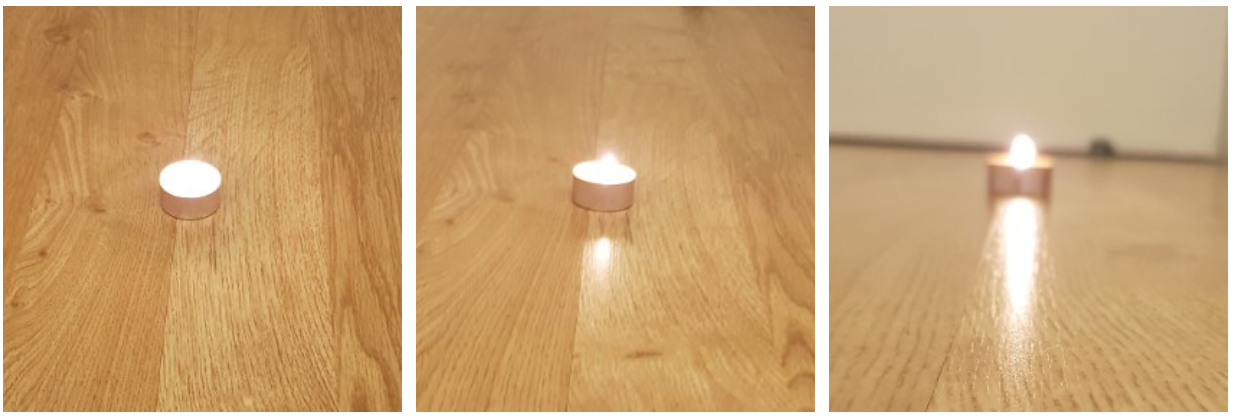
\includegraphics[width=12cm]{FresnelRealLife}
	\caption{The Fresnel effect can be observed in the real world by varying the viewing angle. Taken from~\cite{MarkusLecture}.}
	\label{fig:FresnelRealLife}
\end{figure}

\subsection{Results}

The sampled frames for the two shading models are given in Figure \ref{fig:FresnelResults}.

\begin{figure}[h]
	\centering
	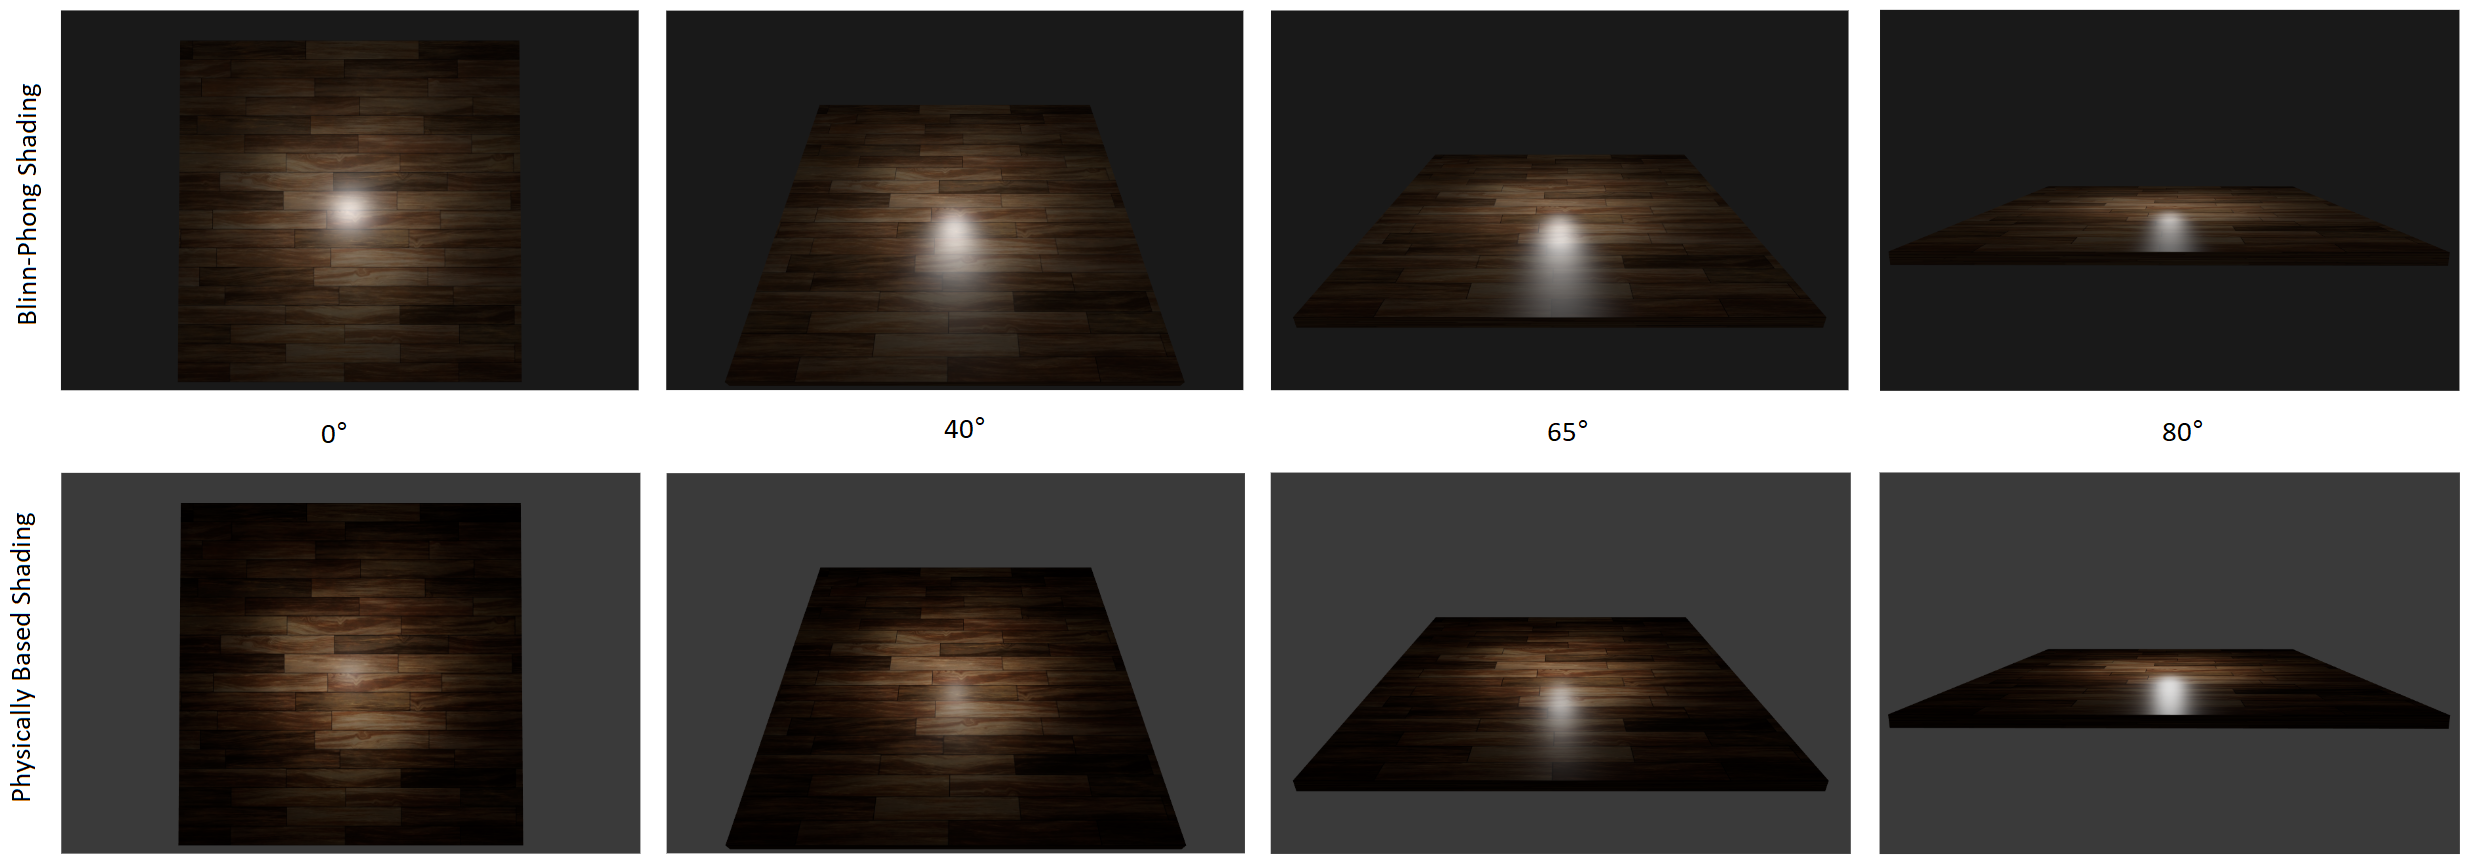
\includegraphics[width=18cm]{FresnelResults}
	\caption{Comparing Blinn-Phong and Physically Based Shading for the presence of the Fresnel effect. Viewing angles are given between the images.}
	\label{fig:FresnelResults}
\end{figure}

\subsection{Analysis}

In the frames rendered using the Blinn-Phong shading model, the wooden floor has a constant specular response over all viewing angles - the Fresnel effect is not being modelled. This is expected, as the Blinn-Phong shading model laid out in equation \ref{eq:BlinnPhong} contains no means of computing the Fresnel reflectance. This poses an issue for artists. They could choose material properties that ensure the specular response of an object is accurate at large viewing angles, but this would have the downside of making the object appear much too specular at smaller viewing angles. This was the approach used for the Blinn-Phong wooden floor material in Figure \ref{fig:FresnelResults}. Alternatively, they could do the opposite, and have more accurate specularity at smaller viewing angles, but sacrifice it at large viewing angles. Either way, a compromise is made that limits the realism of frames rendered using the Blinn-Phong shading model.

In contrast, the physically based shading model is clearly exhibiting the Fresnel effect. At small viewing angles, the wooden floor appears mostly diffuse with only a small specular response. As the angle increases towards \begin{math}90^{\circ}\end{math}, so does the specularity increase. Not only this, but the increase also follows the non-linear behaviour described in section \ref{FresnelReflectance}. This is evidenced by the fact that the specularity does not change between viewing angles \begin{math}0^{\circ}\end{math} and \begin{math}40^{\circ}\end{math}. It is at \begin{math}65^{\circ}\end{math}, and especially \begin{math}80^{\circ}\end{math}, where an increased specular response is observed. The way in which the specular response varies over the PBS frames bears close resemblance to Figure \ref{fig:FresnelRealLife}. The presence of the Fresnel effect is due to the Fresnel reflectance function in equation \ref{eq:SpecularBRDF}, which is implemented in the physically based shading model by means of the Schlick approximation.

The Fresnel effect is a physical phenomena that is accurately modelled in frames rendered by the physically based shading model, and is completely absent in frames rendered by the Blinn-Phong shading model.

\section{Multiple Lights Comparison}

\subsection{Testing Method}

Similar to the previous test, two scenes have been created for the two renderers, and both are arranged identically. A diffuse wooden wall is put just in front of the camera, and attached to it is a light fixture. A varying number of point lights are then all placed where the bulb of the light fixture would be if it existed.

Each Blinn-Phong point light is given the same properties: the \mintinline{cpp}|diffuseComponent| and \mintinline{cpp}|specularComponent| attributes are both set to \begin{math}(1, 1, 1)\end{math}; the \mintinline{cpp}|lightRadius| attribute is set to 10. Likewise, every PBS point light is given the same properties: the \mintinline{cpp}|lightColor| attribute is set to a value of \begin{math}(1, 1, 1)\end{math}; the \mintinline{cpp}|luminousPower| attribute is set to 50; the \mintinline{cpp}|lightRadius| attribute is set to 10. By setting \mintinline{cpp}|luminousPower| to 50, a single PBS point light exhibits an intensity that is similar to a single Blinn-Phong point light.

The test is conducted by varying the number of point lights placed in the scene - from 1 to 10 - and then for each number, sampling the outputted frames of the two renderers.

\subsection{Results}

A subset of the sampled frames for the two shading models are given in Figure \ref{fig:MultipleLightsResultsFrames}. The pixel values of all the rendered frames were converted to HSV triplets and further analysis was performed. Table \ref{tb:MultipleLightsResultsSaturatedPixelValues} gives the number of pixels in the rendered frames that were fully saturated, meaning they had a Value component of 255 and were completely white.

\begin{figure}[h]
	\centering
	\includegraphics[width=18cm]{MultipleLightsResultsFrames}
	\caption{Comparing how the Blinn-Phong and physically based shading models render multiple point lights. The number of point lights present in the scene are given between the images.}
	\label{fig:MultipleLightsResultsFrames}
\end{figure}

\begin{table}
	\noindent\begin{tabular}{|l|l|l|}
		\hline
		\textbf{Point Light Count} & \textbf{Blinn-Phong Shading} & \textbf{Physically Based Shading} \\
		\hline\hline
		\textbf{1} & 0 & 0 \\
		\textbf{2} & 21028 & 0 \\
		\textbf{3} & 83647 & 0 \\
		\textbf{4} & 160152 & 0 \\
		\textbf{5} & 214592 & 0 \\
		\textbf{6} & 249421 & 0 \\
		\textbf{7} & 272263 & 0 \\
		\textbf{8} & 288192 & 0 \\
		\textbf{9} & 301453 & 0 \\
		\textbf{10} & 313752 & 0 \\
		\hline
	\end{tabular}
	\caption{The number of fully saturated pixels in the rendered frames of the two shading models, broken down by number of point lights.}
	\label{tb:MultipleLightsResultsSaturatedPixelValues}
\end{table}

\subsection{Analysis}

A number of issues are evident in the frames rendered using the Blinn-Phong shading model. Table \ref{tb:MultipleLightsResultsSaturatedPixelValues} shows that the number of fully saturated, completely white pixels is substantial. Pixels such as these pose a couple of issues. The first is that they are at maximum brightness, so no matter how many additional lights become incident to the surface, the displayed brightness will not increase. Consider the 21028 pixels that are immediately saturated after just two lights are present in the scene. This means a significant portion of the frame becomes no brighter, even after the number of lights is quadrupled. The second issue is that when neighbouring pixels are completely white, all the detail that existed between them is lost. The top row of Figure \ref{fig:MultipleLightsResultsFrames} shows that this loss of detail manifests itself as unnatural white void that spreads over the image. All of this behaviour is a consequence of the Blinn-Phong renderer effectively ignoring any shaded values that are outside the LDR space by clipping them.

In contrast, Table \ref{tb:MultipleLightsResultsSaturatedPixelValues} shows that the frames rendered using the physically based shading model contain no fully saturated pixels. This means all the pixels have space to further increase in brightness as more point lights become incident to the object surface. As a result, Figure \ref{fig:MultipleLightsResultsFrames} shows a much more natural increase in brightness on the bottom row. Furthermore, a considerable amount of detail is preserved in the brighter regions. These benefits are realised due to the sophisticated tone mapping that is performed by the physically based renderer. This tone mapping is implemented using the ACES operator, which features a sigmoid shape. The sigmoid causes the shaded HDR RGB triplets to be smoothly tapered off at the extremes, meaning fully saturated values being outputted to the display are rare.

Overall, it is clear that the physically based shading model renders the effects of multiple incident lights much more accurately than the Blinn-Phong shading model. Using a physically based shading model therefore has important implications for artists. It gives them more freedom to place lights wherever they wish, without worrying that unnatural effects will occur.

\section{Real Time}

\begin{itemize}
	\item How it's tested
	\begin{itemize}
		\item Perhaps increasing complexities of scenes
	\end{itemize}
	\item Results of those tests (table of frame times)
	\item Discussion of results
\end{itemize}

\subsection{Testing Method}

\subsection{Results}

\subsection{Analysis}
